\documentclass[report]{jlreq}
%%\documentclass[report, a4paper,12pt,left=25mm,right=10mm,top=15mm,bottom=15mm]{jlreq}
\usepackage{array}
\usepackage{multirow}
\usepackage[dvipdfmx]{graphicx} % \resizebox用
\usepackage{subcaption} 

\begin{document}

\title{
スパイラルコア用リボンケーブルの

ダイリップ形状推定方法開発
}
\author{シセ-キ 小林}
\date{2025/08/28}
\maketitle

\chapter{概要}
スパイラルコア用リボン押出を対象とし、異形樹脂押出工程における CAE\footnote{Computer Aided Engineering}手法を検討した。

実製造工程と製品形状を数値化し、物理モデルと統計モデルで記述する方法、およびモデルの逆解析による製造工程最適化方法について説明する。

\chapter{背景}
スパイラルコア({\small 以下 "SC" と略})は、電力ケーブル接続部の絶縁処理部材 RBJ\footnote{Rubber Block Joint - 電力用ケーブル(主にCVケーブル)を接続する際に使われる、ゴムブロック絶縁型のジョイント(中間接続部材)} の装着時に使用される円筒状の部材である。この SC は SC 用リボンをらせん({\small スパイラル})状に嵌合させ形成されており、嵌合時の強度と安定性を確保するために適切な断面形状が指定されている\footnote{参考 : 特開2006-289791}({\small 図\ref{fig:SC_M-6-4} , \ref{fig:SC_M-10-7} 参照})\footnote{"スパイラルコア用リボン購入仕様書", ATS-SS-060697H号 より抜粋}。

\begin{figure}
  \centering
    \begin{minipage}{0.45\columnwidth}
    \centering
    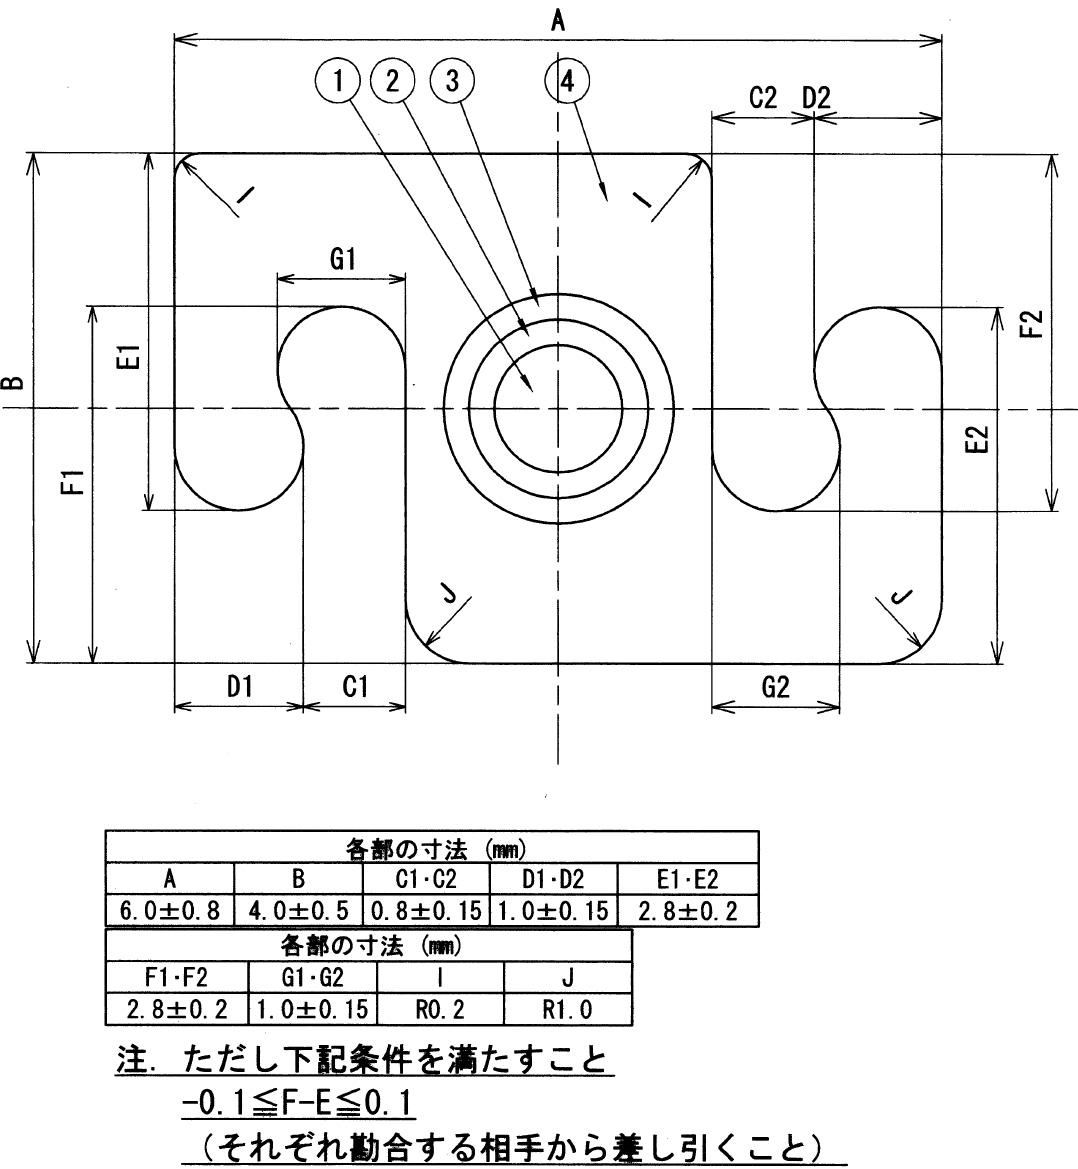
\includegraphics[width=\columnwidth]{SC_M-6-4.jpg}
    \caption{SC M-6-4 図面}
    \label{fig:SC_M-6-4}
  \end{minipage}
  \hspace{5mm}
  \begin{minipage}{0.45\columnwidth}
    \centering 
    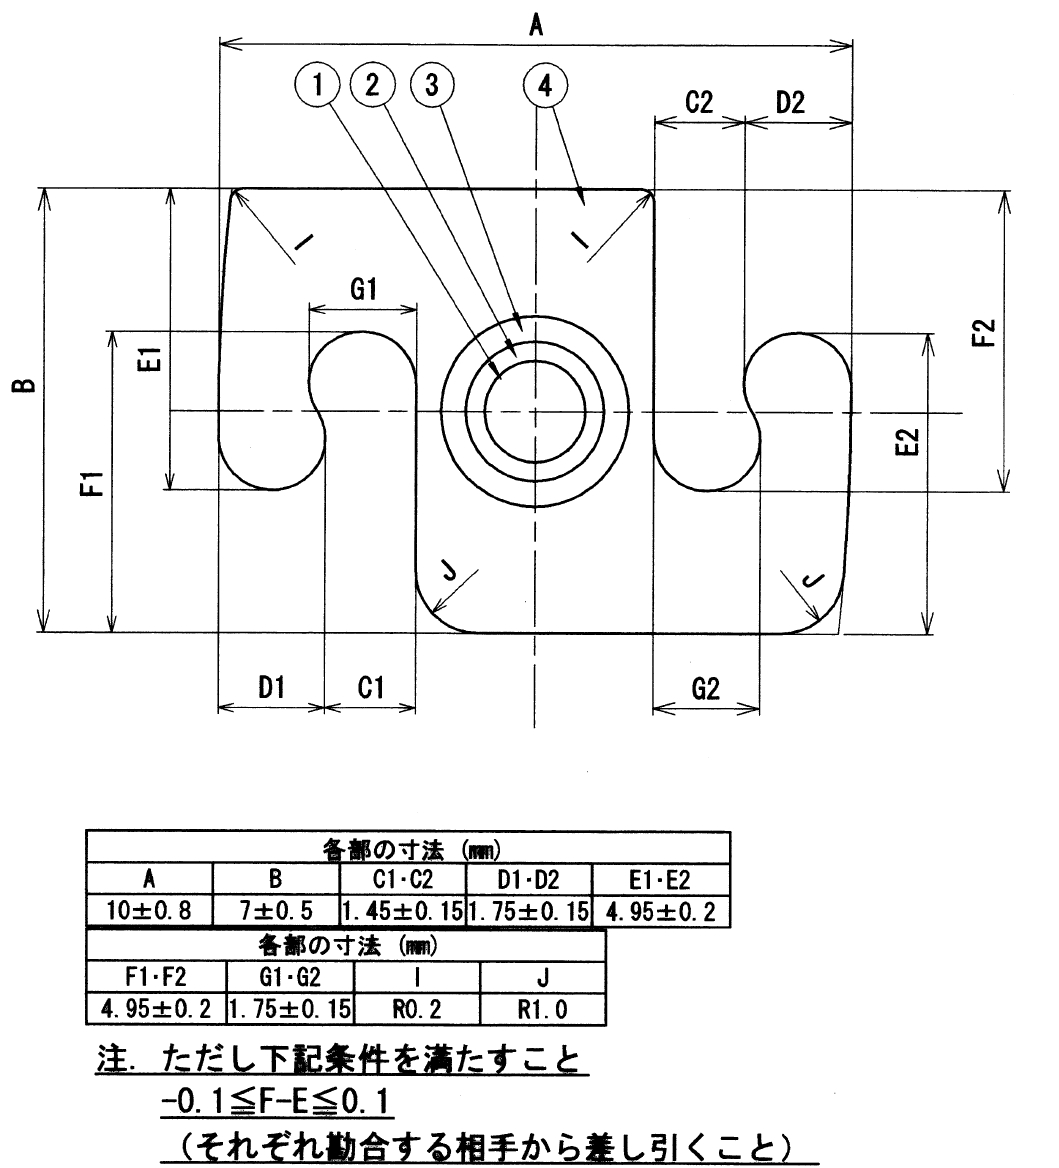
\includegraphics[width=\columnwidth]{SC_M-10-7.jpg}
    \caption{SC M-10-7 図面}
    \label{fig:SC_M-10-7}
  \end{minipage}
\end{figure} 

この SC 用リボンケーブルはこれまで UEXC\footnote{宇部エクシモ株式会社 https://www.ube-exsymo.co.jp/}社に外注していたが、2025年3月をもって製造から撤退することとなったため、2026年10月までにSWCC社の内製化に移行することとなった。

\chapter{目的}
内製化移行計画において難易度が高い課題の一つにダイス設計がある。

樹脂押出工程において、ダイス出口から吐出する溶融樹脂は柔らかい流体であるため、冷却固化するまでに様々な外的要因({\small 例えば吐出口の流速分布や重力の影響など})により変形する。

そのため、ダイス設計はその「押出工程における樹脂変形挙動」を考慮し製品設計からダイス形状を推定する\textgt{逆解析問題}といえる。

従来この問題解決は、"複数のダイス形状" と "それを用いた押出製品の形状" を目視で比較し、ダイス形状変化に対する製品形状変化から傾向を読み取ることで行われていた。
しかし、多分に解析者の主観や経験の影響を受ける手法であり、属人化が強いうえ効率が良いと言えなかった。

本検討の第一の目的は、この "人手による逆解析" をシミュレーションやインフォマティックスといった数値解析・情報工学を駆使することで\textgt{データ駆動型逆解析}とする要素技術確立およびその要素技術の組合せによるソリューション開発を行うことである。

そして最終的な目的は、そのソリューションを用いることで本内製化プロジェクトのスケジュールを遅延なく進めることである。


\chapter{実験方法/解析方法}
\section{本検討の全体像}
本検討ではソリューション({\small 逆解析})本体を物理モデルと数学モデルの組合せで実現する。

そして、このソリューションの妥当性確認は試作データとの比較により行う。

以下に、物理モデル - 数学モデル - 実測({\small 値}) の連携方法について示す。

\section{形状表現}
物理モデル - 数学モデル - 実測(値)のそれぞれにおいて、製品とダイリップの輪郭形状を比較するためには数学的表現を定義する必要がある。

今回は輪郭の多角形表現を用いた。({\small 図\ref{fig:polygon}})

\begin{figure}
  \centering
    \begin{subfigure}{0.45\columnwidth}
      \centering
      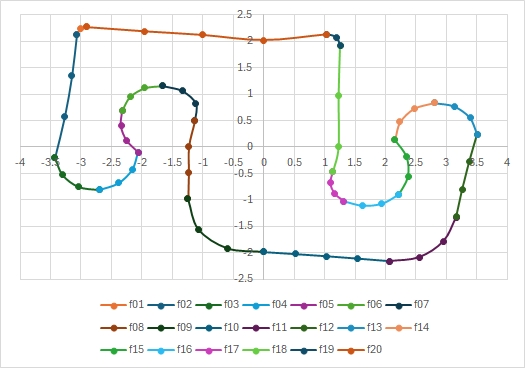
\includegraphics[width=\columnwidth]{D05_DieLip.jpg}
      \caption{SC M-6-4 UEXC ダイリップ}
      \label{fig:hidari}
    \end{subfigure}
    \hspace{5mm}
    \begin{subfigure}{0.45\columnwidth}
      \centering
      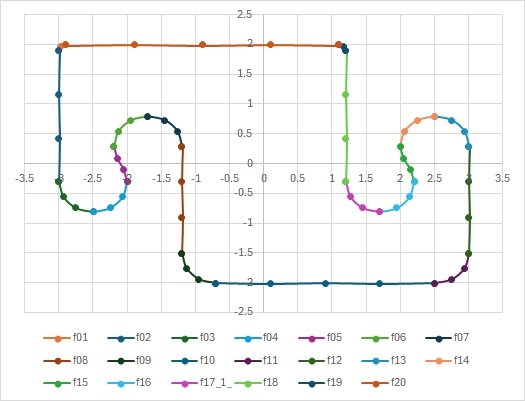
\includegraphics[width=\columnwidth]{SC_M-6-4_polygon.jpg}
      \caption{SC M-6-4 製品} 
      \label{fig:SC_M-6-4_polygon}
    \end{subfigure}
    \caption{多角形表現}
    \label{fig:polygon} 
\end{figure} 

ダイリップ、製品の両輪郭形状は特徴的な20辺に分割し、それぞれの辺を2~4分割することで60角形としている。

\newpage

\section{シミュレーション}
本報では物理現象に基づく数値解析をシミュレーションと呼ぶ。

想定している物理現象を以下に示す。

\begin{enumerate}
  \item ダイス内流路
  \begin{enumerate}
    \item 伝熱解析(壁面や線材との間の伝熱)
    \item 流体解析(固定壁面で定義された流路内流れ)
  \end{enumerate}
  \item 押出機外流路
  \begin{enumerate}
    \item 流体解析1 (出口における速度分布に基づく断面内流れ)
    \item 流体解析2 (重力影響による流れ)
    \item 流体解析3 (上記 1, 2の影響による自由表面の変形)
    \item 伝熱解析(空冷や水冷による断面内温度分布)
    \item 構造解析(温度と線膨張係数から求めた体積変化)
    \item 流体解析4 (体積変化の影響による自由表面の変形)
  \end{enumerate}
\end{enumerate}


\subsection{物理モデル}
想定している物理現象は、「自由表面を考慮した流体」という物理モデルで取り扱う。

ただし、空冷や水冷による冷却({\small 物理現象 2(d)})を解析するための表面熱伝達率設定は別途熱流体解析を行った。({\small 頁の関係で本報では省略する})

\subsection{流路形状}
流路形状はダイリップ形状を引き延ばした多角柱状とした。流路中心には1次被覆を考慮した線材径に相当する円筒状領域が設けてある。

ダイス内流路長さは40[mm]({\small 図\ref{fig:geometry_mesh}(a)の濃い緑色の領域})、ダイス外流路長さは50[mm]({\small 標準的な変形解析用})、150[mm]({\small 長時間で生じる変形解析用})とした({\small 図\ref{fig:geometry_mesh}(a)の薄い水色の領域})。

\begin{figure}
  \centering
    \begin{subfigure}{0.45\columnwidth}
      \centering
      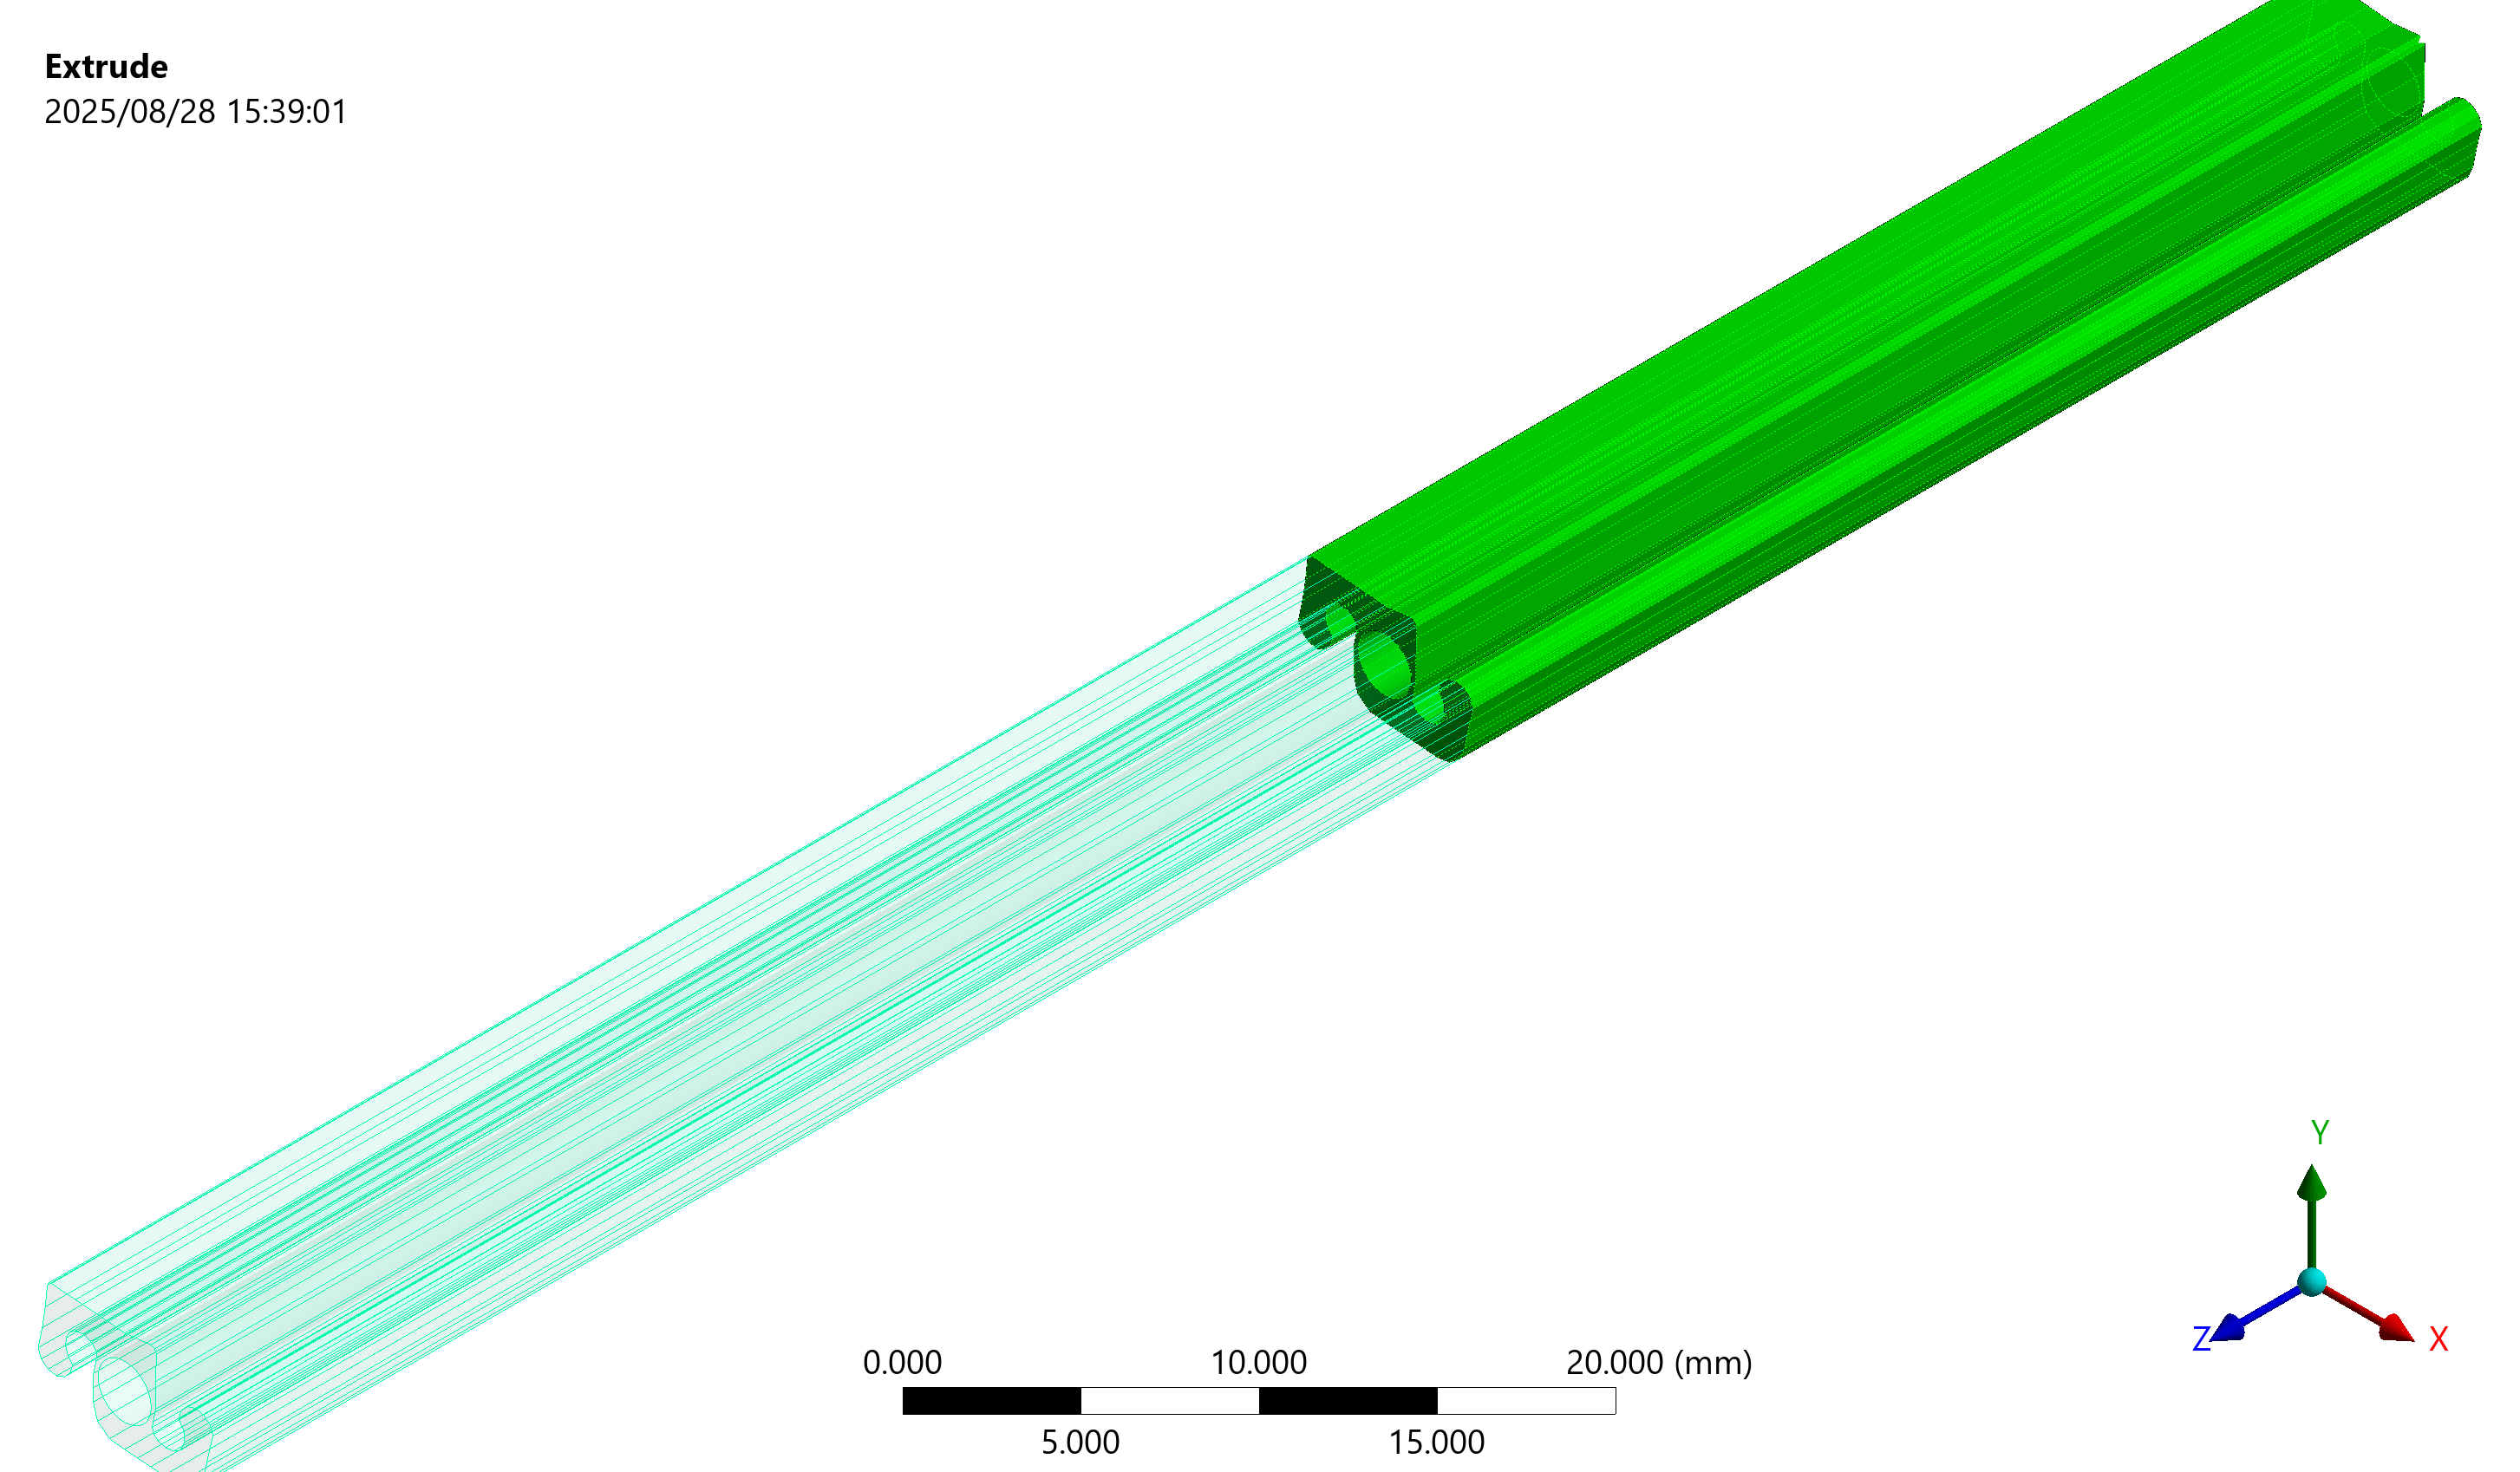
\includegraphics[width=\columnwidth]{2508221_mesh.jpg}
      \caption{流路全体}
      \label{fig:mesh1}
    \end{subfigure}
    \hspace{5mm}
    \begin{subfigure}{0.4\columnwidth}
      \centering
      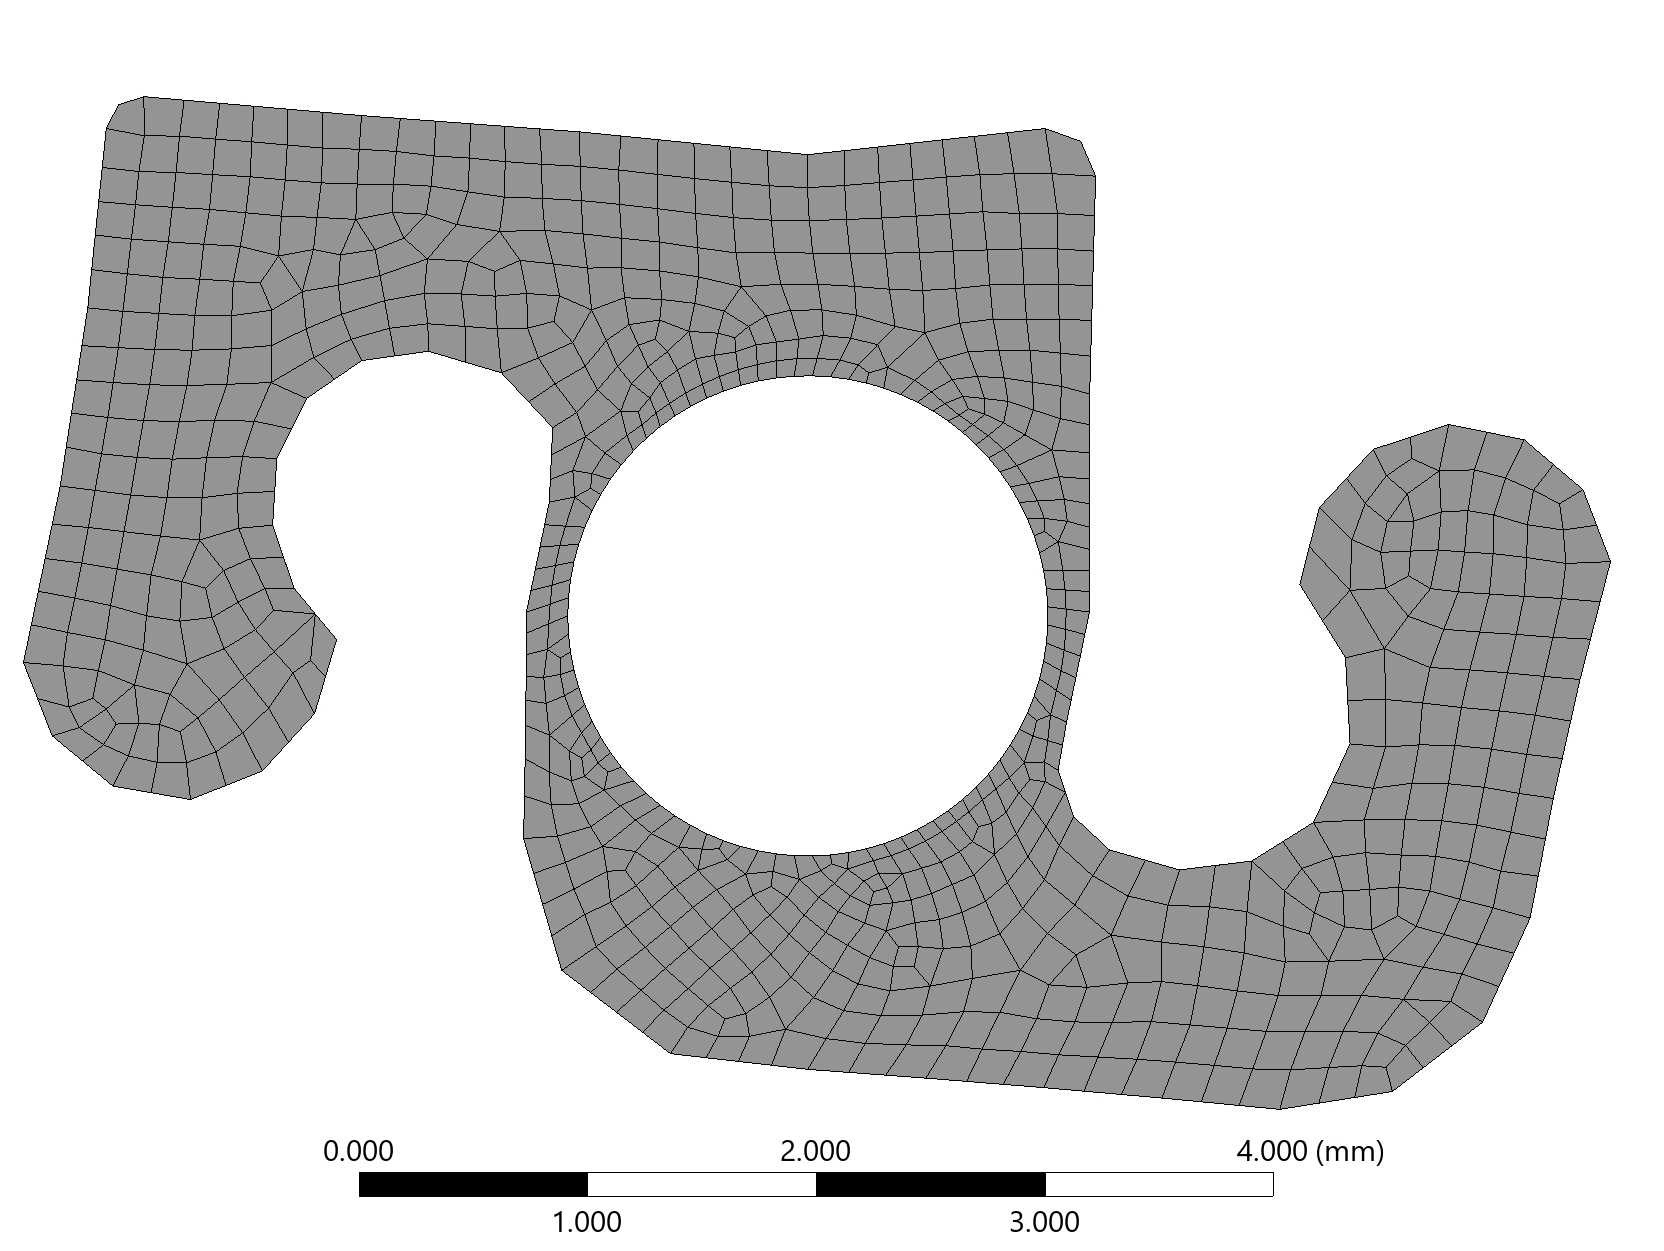
\includegraphics[width=\columnwidth]{2508222_mesh.jpg}
      \caption{断面拡大} 
      \label{fig:mesh2}
    \end{subfigure}
    \caption{流路形状およびメッシュ({\small SC M-6-4})}
    \label{fig:geometry_mesh} 
\end{figure} 



\subsection{境界条件}

\begin{itemize}
  \item 樹脂入口 : 図\ref{fig:geometry_mesh}(a) のZ軸マイナス側に設定。基本的に線速に基づく速度境界としている。
  \item 芯線表面 : 速度境界。滑り無し。線速をz+ベクトルとして設定。
  \item ダイス内流路表面 : 固定境界。滑り無し。現時点では断熱境界として取り扱っている。
  \item ダイス外流路表面 : 自由表面。図\ref{fig:polygon}に基づいて面({\small 辺})毎に境界温度と熱伝達率を定義。
\end{itemize}

\subsection{材料物性}
使用材料 : Hizex6300M

物性値を以下に示す。
\begin{table}
\centering
\caption[Hizex6300M物性値]{Hizex6300M物性値}  
\label{Hizex6300M}
\setlength{\tabcolsep}{5pt}
\begin{tabular}{|c|r|l|}\hline
物性値 & 数値 & 備考\\ \hline
密度[$kg/m^3$] & 951 & 固体での値\\ \hline
線膨張係数[$1/K$] & $1.2\times10^{-4}$ &固体での値\\ \hline
\end{tabular}
\end{table}% 

粘度は擬塑性流体として取り扱っており、せん断速度依存性はCross則、温度依存性は Arrhenius則で表現している。

\begin{table}
\centering
\caption[Hizex6300M粘度]{Hizex6300M粘度}  
\label{Hizex6300M_visco}
\setlength{\tabcolsep}{5pt}
\begin{tabular}{|c|c|l|}\hline
せん断速度依存性 & $\eta=\frac{\eta_{0}}{1+(\lambda\cdot\dot{\gamma})} $ &  Cross則\\ \hline
温度依存性 & $H(T)=exp(\alpha(\frac{1}{T-T_{0}} - \frac{1}{T_{\alpha}-T_{0}}))$ & Arrhenius則\\ \hline
\end{tabular}
\end{table}% 


\subsection{解析用ソフトウェア}
ANSYSソフトウェアスイートを用いている。バージョンは 2025 R1。
\begin{itemize}
  \item 熱流体解析ソルバー1 : ANSYS Polyflow - 自由表面変形を考慮した流体解析
  \item 熱流体解析ソルバー2 : ANSYS Fluent - 表面の熱伝達率計算用
  \item モデラ― : ANSYS DesignModeler
  \item メッシャー : ANSYS Meshing
\end{itemize}



\subsection{解析用ハードウェア}
ハードウェアの基本仕様を以下に示す。

\begin{itemize}
  \item プロセッサ	Intel(R) Core(TM) Ultra 9 285K   3.70 GHz
  \item 実装 RAM	192 GB
  \item Windows 11 Pro Version 23H5
\end{itemize}



\section{インフォマティックス}
「インフォマティックス」という単語は文脈によりいろいろな意味で用いられる。

本報ではシミュレーション({\small 物理モデル表現})以外の数理モデル表現をすべてインフォマティックスに含まれるものとして取り扱うことにする。

すなわちデータ空間内の分布傾向を把握すること、それに基づく逆解析による推定、試作結果に基づく実測値と推定値とのずれに基づくフィードバック処理、またシミュレーションを含めすべての連携で最適形状の推定を行うことなどをインフォマティックスとして取り扱う。

話を単純にするため、ここでは「シミュレーションと試作のデータ傾向の確認」「逆解析」および「形状最適化」について説明する。

\subsection{データ傾向の確認}


\subsection{逆解析}
\subsection{形状最適化}


\section{試作}



\chapter{結果}
実験・シミュレーションの結果を簡潔に記す
箇条書きもOK
\chapter{考察 }
実験・シミュレーションの考察を簡潔に記す
箇条書きもOK
\chapter{結論}
結論を記す
目的と結論が一対になっているかを確認する
箇条書きもOK
\chapter{今後の進め方}
   今後の進め方を記す
   箇条書きもOK
\chapter{参考報告書・文献}
   関係する報告書・文献を記す


\end{document}